\graphicspath{{Images/}}

\section{LCSR for $D_{s}^{+}\to\eta^{(\prime)}$}

\subsection{Correlation Function}

LCSR starts with the correlation function Eq.\ref{eq:correlation_function}.
\begin{equation}
    \Pi_\mu(p, q)=i \int d^4 x e^{i q x}\left\langle \eta^{(\prime)}(p)\left|\mathrm{T}\left\{j_{\mu,1}(x), j_{2}(0)\right\}\right| 0\right\rangle
    \label{eq:correlation_function}
\end{equation}

In reference~\cite{JHEP1}, the currents entering the correlation function are defined as shown in Table~\ref{tab:Currents}.

\begin{table}[htbp]
    \centering
    \caption{Currents entering the correlation function\cite{JHEP1}.}
    \vspace{4mm}
    \begin{tabular}{c | c c}
        \hline \hline
        \textbf{Decay}                                                                  & \textbf{Interpolation current}                                                                           & \textbf{Weak current} \\
        \hline
        \multirow{2}{*}{$D_{s}^{+}\rightarrow\eta^{(\prime)}l^{+}\nu_{l}$}              &
        \multirow{2}{5cm}{~~~~$j_{2} = j_{D_s^{+}}^{\dagger}=m_c \bar{c} i \gamma_5 s$} &
        $j_{\mu,1} = V_\mu^{\left(\eta, \eta^{\prime}\right)}=\bar{s} \gamma_\mu c$                                                                                                                                        \\
                                                                                        &
                                                                                        & $\Tilde{j}_{\mu,1} = \Tilde{V}_\mu^{\left(\eta, \eta^{\prime}\right)}=\bar{s} \sigma_{\mu\nu} q^{\nu} c$                         \\
        \hline\hline
    \end{tabular}
    \label{tab:Currents}
\end{table}

The Feynman diagram corresponding to the formula is shown in fig.\ref{fig:feynman1}.

\begin{figure}[!hpt]\centering
    \rotatebox{90}{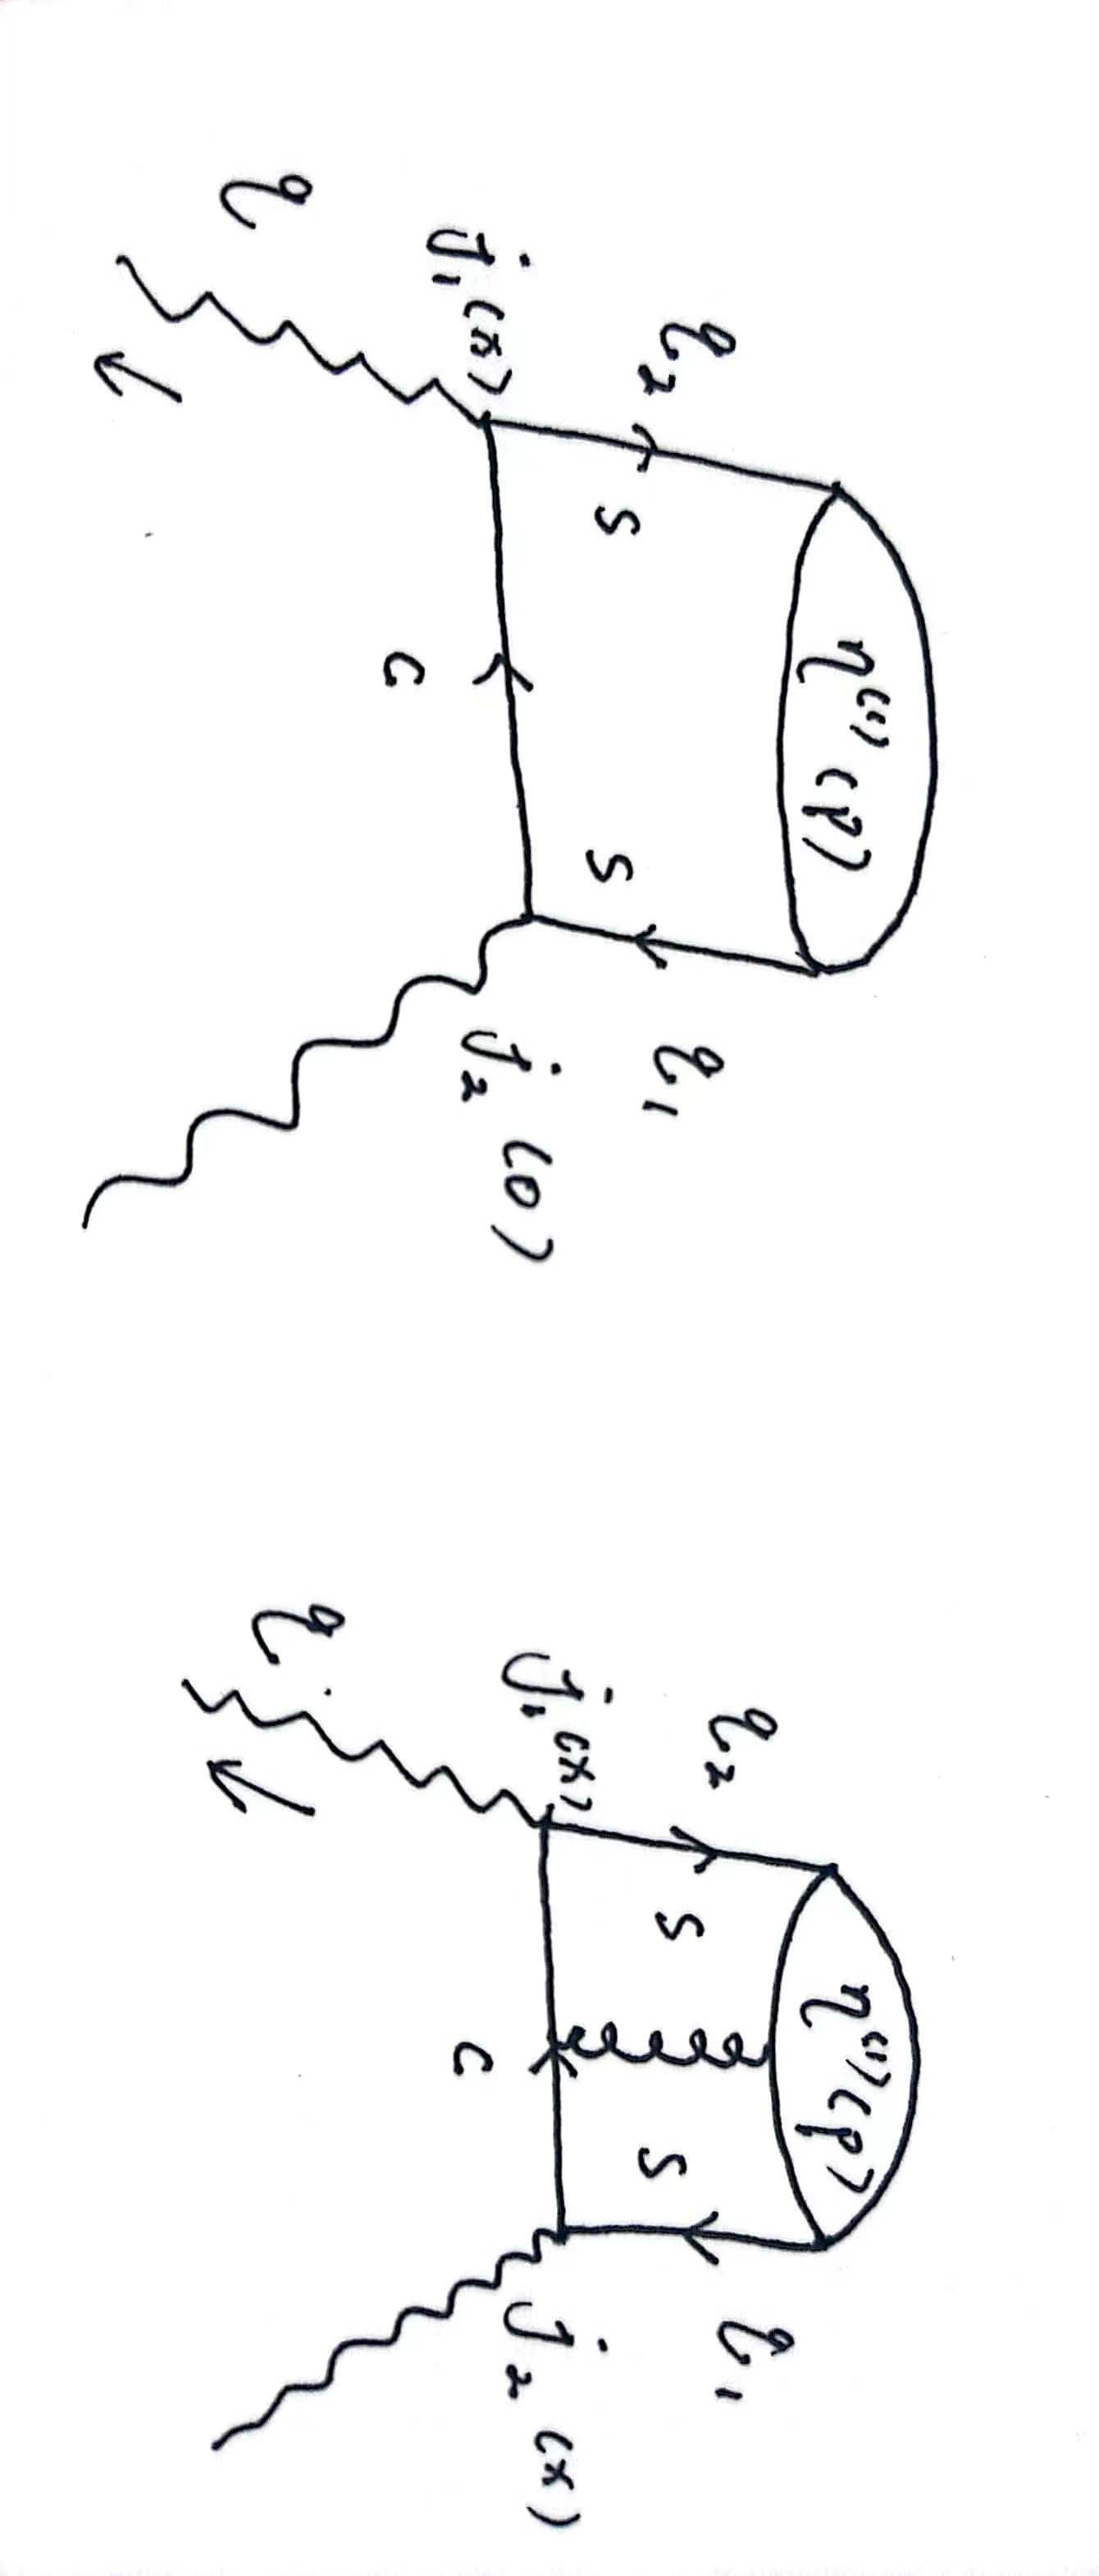
\includegraphics[width=0.3\textwidth]{image/feynman.jpg}}
    \caption{Diagrams corresponding to the leading-order terms in the hard-scattering amplitudes
        involving the two-particle (left) and three-particle (right)}
    \label{fig:feynman1}
\end{figure}

It has been showen by Källén and Lehmann~\cite{Kallen1952, Lehmann1954} quite a long time ago that the two-point correlation functions obey dispersion relation:
\begin{equation}
    \Pi_\mu(p, q)= \int_{0}^{\infty} dt\, \rho_{\mu}(t)\frac{1}{t-(p+q)^{2}-i\epsilon}
\end{equation}

For $(p+q)^{2}>0$, we have
\begin{equation}
    \begin{array}{rl}
        \Pi_\mu(p, q) & = \mathcal{P} \int_{0}^{\infty} dt\, \rho_{\mu}(t)\frac{1}{t-(p+q)^{2}} + i\pi\rho_{\mu}((p+q)^{2}) \\
                      & = \mathrm{Re}\Pi_\mu(p, q) + \mathrm{Im}\Pi_\mu(p, q)
    \end{array}
    \label{eq:dispersion_relation_real}
\end{equation}

Clearly, $\mathrm{Im}\Pi_\mu(p, q)$ has a corresponding relationship with $\pi\rho_{\mu}((p+q)^{2})$, the spectral function density $\rho_{\mu}((p+q)^{2})$ is a scalar function of the Lorentz invariant $(p+q)^{2}$.
\begin{equation}
    \rho_{\mu}(t) = \frac{1}{\pi} \mathrm{Im}\Pi_\mu(t) \equiv \sum_{\Gamma}^{} \langle \eta^{(\prime)}|j_{\mu,1}|\Gamma\rangle \langle \Gamma|j_{2}|0\rangle (2 \pi)^4 \delta^{(4)}\left(q-p_{\Gamma}\right)
\end{equation}

Given the definition of $\mathrm{Im}\Pi_\mu(t)$, naturally, we have
\begin{equation}
    \Pi_\mu(p, q)= \frac{1}{\pi} \int_{0}^{\infty} dt\, \frac{\mathrm{Im}\Pi_\mu(t)}{t-(p+q)^{2}-i\epsilon}
    \label{eq:dispersion_relation}
\end{equation}


\subsection{Hadron Representation}
After inserting a complete set of hadronic states, specifically $|D_{s}^{+}(p+q)\rangle$, we have $(p+q)^{2} \geq m_{Ds}$ in the physical region.
\begin{equation}
    \begin{aligned}
        \Pi_\mu(p, q)^{hadron} & = i \int d^4 x e^{i q x}\left\langle \eta^{(\prime)}(p)\left|\mathrm{T}\left\{j_{1}(x), j_{2}(0)\right\}\right| 0\right\rangle + \frac{1}{\pi}  \int_{s_0}^{\infty} dt\, \frac{\mathrm{Im}\Pi_\mu^{hadron}(t)}{t-(p+q)^{2}-i\epsilon}              \\
                               & = \frac{-i m_{D_s}^2 f_{D_s}[2 f_{D_{(s)} \eta^{(\prime)}}^{+}\left(q^2\right) p_\mu+\left(f_{D_{(s)} \eta^{(\prime)}}^{+}\left(q^2\right)+f_{D_{(s)} \eta^{(\prime)}}^{-}\left(q^2\right)\right)q_\mu]}{(m_c+m_s)[m^{2}_{D_{s}^{+}} - (p+q)^{2}]} \\
                               & \quad + \frac{1}{\pi} \int_{s_0}^{\infty} dt\, \frac{\mathrm{Im}\Pi_{+}^{hadron}(t,q^{2})p_{\mu} + \mathrm{Im}\Pi_{-}^{hadron}(t,q^{2})q_{\mu}}{t-(p+q)^{2}-i\epsilon}
    \end{aligned}
    \label{eq:hadron_rep}
\end{equation}
where $f_{D_{(s)} \eta^{(\prime)}}^{+}$ and $f_{D_{(s)} \eta^{(\prime)}}^{-}$ are the form factors defined as Eq.\ref{eq:form_factor}:
\begin{equation}
    \begin{aligned}
         & \left\langle \eta^{(\prime)}|j_{\mu,1}|D_{s}^{+}(p+q)\right\rangle=2 f_{D_{(s)} \eta^{(\prime)}}^{+}\left(q^2\right) p_\mu+\left(f_{D_{(s)} \eta^{(\prime)}}^{+}\left(q^2\right)+f_{D_{(s)} \eta^{(\prime)}}^{-}\left(q^2\right)\right) q_\mu,
    \end{aligned}
    \label{eq:form_factor}
\end{equation}

\subsection{Quark Representation}
Computed in the perturbative theory with the help of OPE technique at the deep Euclidean region $(p^{2}, q^{2} = -Q^{2} \ll 0)$, we have:
\begin{equation}
    \begin{aligned}
        \Pi_\mu(p, q)^{OPE} & = i \int d^4 x e^{i q x}\left\langle \eta^{(\prime)}(p)\left|\mathrm{T}\left\{j_{\mu,1}(x), j_{2}(0)\right\}\right| 0\right\rangle                                                                                                                                                                                                                                      \\
                            & = i \int d^4 x e^{i q x}\left\langle \eta^{(\prime)}(p)\left|\mathrm{T}\left\{\bar{s}(x) \gamma_\mu c(x), \bar{c}(0) i \gamma_5 s(0)\right\}\right| 0\right\rangle                                                                                                                                                                                                      \\
                            & = i \int d^4 x e^{i q x}\left\langle \eta^{(\prime)}(p)\left|\mathrm{T}\left\{\bar{s}_{\alpha}(x) \left[\gamma_{\mu}\right]_{\alpha\alpha^{\prime}} c_{\alpha^{\prime}}(x), \bar{c}_{\beta}(0) \left[i \gamma_{5}\right]_{\beta\beta^{\prime}} s(0)_{\beta^{\prime}}\right\}\right| 0\right\rangle                                                                      \\
                            & = i \int d^4 x e^{i q x}\left\langle \eta^{(\prime)}(p)\left| \mathrm{T}\left\{\bar{s}_{\alpha}(x)s(0)_{\beta^{\prime}}\right\} \right| 0\right\rangle \left\langle 0\left| \mathrm{T}\left\{c_{\alpha^{\prime}}(x) \bar{c}_{\beta}(0)\right\} \right| 0\right\rangle \left[\gamma_{\mu}\right]_{\alpha\alpha^{\prime}} \left[i \gamma_{5}\right]_{\beta\beta^{\prime}}
    \end{aligned}
    \label{eq:quark_rep}
\end{equation}
Where $\left\langle 0\left| \mathrm{T}\left\{c_{\alpha^{\prime}}(x) \bar{c}_{\beta}(0)\right\} \right| 0\right\rangle \equiv S_{c}^{\alpha^{\prime}\beta}\left(x, 0, m_c\right)$ is the full propagator of c quark. The light-cone expansion of the quark propagator in the external gluon field is made in ref~\cite{BalitskyBraun1989}. The propagator receives contributions from higher Fock states proportional to the condensates of the operators $\bar{q}Gq$, $\bar{q}GGq$ and $\bar{q}q\bar{q}q$. We neglect contributions with two gluons as well as four quark operators due to the fact that their contributions are small ~\cite{BraunFilyanov1990}. In this approximation the $S_c\left(x, 0, m_c\right)$ is given as:


\begin{equation}
    \begin{aligned}
        S_{c}\left(x, 0, m_c\right) & =\int \frac{\mathrm{d}^4 k}{(2 \pi)^4} \mathrm{e}^{-\mathrm{i} k x} \frac{\slashed{k}+m_c}{k^2-m_c^2}                                                                                                     \\
                                    & \quad -\mathrm{i} g_s \int \frac{\mathrm{d}^4 k}{(2 \pi)^4} \mathrm{e}^{-\mathrm{i} k x} \int_0^1 \mathrm{d} u\Biggl[ \frac{1}{2} \frac{\slashed{k}+m_c}{(m_c^2-k^2)^2} G_{\mu \nu}(u x) \sigma^{\mu \nu} \\
                                    & \quad +\frac{1}{m_c^2-k^2} u x_\mu G^{\mu \nu}(u x) \gamma_\nu + \cdots \Biggr]                                                                                                                           \\
                                    & ~~~~~~~~~~~~~~~~~~\cdots\text{(Fourier transform)}\cdots                                                                                                                                                  \\
                                    & =\frac{-i m_c^2}{4 \pi^2}\Biggl[\frac{K_1\left(m \sqrt{|x^2|}\right)}{\sqrt{|x^2|}}+i \frac{\slashed{x}}{|x^2|} K_2\left(m_c \sqrt{|x^2|}\right)\Biggr]                                                   \\
                                    & \quad -\frac{i g_s}{16 \pi^2} \int_0^1 d u\Biggl[ m_c K_0\left(m_c \sqrt{|x^2|}\right)(G \cdot \sigma)                                                                                                    \\
                                    & \quad +\frac{i m_c}{\sqrt{|x^2|}} K_1\left(m_c \sqrt{|x^2|}\right)\Biggl(\slashed{x} (G \cdot \sigma)-4 i u x_\mu G^{\mu \nu} r_\nu\Biggr)+\cdots \Biggr]                                                 \\
    \end{aligned}
    \label{eq:propagator_ccbar}
\end{equation}

where $G{\mu\nu}$ is the gluonic field strength tensor and $g_s$ is the strong coupling constant, $K_0\left(m_c \sqrt{|x^2|}\right), K_1\left(m_c \sqrt{|x^2|}\right)$ and $K_2\left(m_c \sqrt{|x^2|}\right)$ are the Bessel functions. Simplify Eq.\ref{eq:quark_rep}:
% \begin{equation}
%     \begin{aligned}
%         \Pi_\mu(p, q)^{OPE} & = i \int d^4 x e^{i q x}\left\langle \eta^{(\prime)}(p)\left|\mathrm{T}\left\{j_{\mu,1}(x), j_{2}(0)\right\}\right| 0\right\rangle                                                                                                                                                                                                                                      \\
%         & = i \int d^4 x e^{i q x}\left\langle \eta^{(\prime)}(p)\left| \mathrm{T}\left\{\bar{s}_{\alpha}(x)s(0)_{\beta^{\prime}}\right\} \right| 0\right\rangle  \left[\gamma_{\mu}\right]_{\alpha\alpha^{\prime}} \left[i \gamma_{5}\right]_{\beta\beta^{\prime}} \times \int \frac{\mathrm{d}^4 k}{(2 \pi)^4} \mathrm{e}^{-\mathrm{i} k x} \frac{\not k+m_c}{k^2-m_c^2}\\
%         & \quad +\mathrm{i} g_s \int d^4 x e^{i q x}\left\langle \eta^{(\prime)}(p)\left| \mathrm{T}\left\{\bar{s}_{\alpha}(x)s(0)_{\beta^{\prime}}\right\} \right| 0\right\rangle  \left[\gamma_{\mu}\right]_{\alpha\alpha^{\prime}} \left[i \gamma_{5}\right]_{\beta\beta^{\prime}} \\
%         & \quad \times \int \frac{\mathrm{d}^4 k}{(2 \pi)^4} \mathrm{e}^{-\mathrm{i} k x} \int_0^1 \mathrm{~d} u\left[\frac{1}{2} \frac{\not k+m_c}{\left(m_c^2-k^2\right)^2} G_{\mu \nu}(u x) \sigma^{\mu \nu}+\frac{1}{m_c^2-k^2} u x_\mu G^{\mu \nu}(u x) \gamma_\nu\right]
%     \end{aligned}
%     \label{eq:quark_rep_01}
% \end{equation}
\begin{equation}
    \begin{aligned}
        \Pi_\mu(p, q)^{OPE} & = i \int d^4 x e^{i q x}\left\langle \eta^{(\prime)}(p)\left|\mathrm{T}\left\{j_{\mu,1}(x), j_{2}(0)\right\}\right| 0\right\rangle                                                                                                                        \\
                            & = i \int d^4 x e^{i q x}\left\langle \eta^{(\prime)}(p)\left| \mathrm{T}\left\{\bar{s}_{\alpha}(x)s(0)_{\beta^{\prime}}\right\} \right| 0\right\rangle  \left[\gamma_{\mu}\right]_{\alpha\alpha^{\prime}} \left[i \gamma_{5}\right]_{\beta\beta^{\prime}} \\
                            & \quad \times \Biggl\{ \frac{-i m_c^2}{4 \pi^2}\left[\frac{K_1\left(m \sqrt{|x^2|}\right)}{\sqrt{|x^2|}}+i \frac{\slashed{x}}{|x^2|} K_2\left(m_c \sqrt{|x^2|}\right)\right]                                                                               \\
                            & \quad -\frac{i g_s}{16 \pi^2} \int_0^1 d u\left[m_c K_0\left(m_c \sqrt{\left| x^2\right|}\right)(G \cdot \sigma)+\frac{i m_c}{\sqrt{|x^2|}} K_1\left(m_c \sqrt{|x^2|}\right)\slashed{x} (G \cdot \sigma) + \cdots\right]  \Biggr\}_{\alpha^{\prime}\beta}
    \end{aligned}
    \label{eq:quark_rep_01}
\end{equation}
from the above,
\begin{equation}
    \begin{aligned}
        \Pi_\mu(p, q)^{OPE} & = \frac{1}{4 \pi^2} \int d^4 x e^{i q x}\left\langle \eta^{(\prime)}(p)\left| \mathrm{T}\left\{\bar{s}_{\alpha}(x)s(0)_{\beta^{\prime}}\right\} \right| 0\right\rangle  \left[\gamma_{\mu}\right]_{\alpha\alpha^{\prime}} \left[i \gamma_{5}\right]_{\beta\beta^{\prime}}                                    \\
                            & \quad \times \left[\frac{m_c^{2}K_1\left(m \sqrt{|x^2|}\right)}{\sqrt{|x^2|}} + i \frac{ \slashed{x} m_c^{2}K_2\left(m_c \sqrt{|x^2|}\right)}{|x^2|}\right]_{\alpha^{\prime}\beta}                                                                                                                           \\
                            & + \frac{1}{4 \pi^2} \int d^4 x e^{i q x} \int_0^1 d u\left\langle \eta^{(\prime)}(p)\left| \mathrm{T}\left\{\bar{s}_{\alpha}(x) g_s G_{\lambda \tau} s(0)_{\beta^{\prime}}\right\} \right| 0\right\rangle  \left[\gamma_{\mu}\right]_{\alpha\alpha^{\prime}} \left[i \gamma_{5}\right]_{\beta\beta^{\prime}} \\
                            & \quad \times  \sigma^{\lambda \tau} \left[ \frac{m_c K_0\left(m_c \sqrt{\left| x^2\right|}\right)}{4} + \frac{i \slashed{x} m_c K_1\left(m_c \sqrt{|x^2|}\right)}{4\sqrt{|x^2|}} + \cdots \right]_{\alpha^{\prime}\beta}.
    \end{aligned}
    \label{eq:quark_rep_02}
\end{equation}
In the Eq.\ref{eq:quark_rep_02}, the matrix element inside the Dirac brackets is provided by the LCDA\cite{BallBraunLenz2006}:

\begin{equation}
    \begin{aligned}
         \left\langle\eta(p)\left|\bar{q}_\omega^i\left(x_1\right) q_{\xi}^j\left(x_2\right)\right| 0\right\rangle_{x^2 \rightarrow 0}                                                                                                      \\
         & \hspace{-4cm} = \frac{i \delta^{i j}}{12} f_\eta \int_0^1 d u e^{i u p \cdot x_1+i \bar{u} p \cdot x_2}\left(\left[\not p \gamma_5\right]_{\xi \omega} \varphi_\eta(u)-\left[\gamma_5\right]_{\xi \omega} \mu_\eta \phi_{3 \eta}^p(u)\right.    \\
         & \hspace{-4cm} +\frac{1}{6}\left[\sigma_{\beta \tau} \gamma_5\right]_{\xi \omega} p_\beta\left(x_1-x_2\right)_\tau \mu_\eta \phi_{3 \eta}^\sigma(u)+\frac{1}{16}\left[\not p \gamma_5\right]_{\xi \omega}\left(x_1-x_2\right)^2 \phi_{4 \eta}(u) \\
         & \hspace{-4cm} \left.-\frac{i}{2}\left[\left(\not x_1-\not x_2\right) \gamma_5\right]_{\xi \omega} \int_0^u \psi_{4 \eta}(v) d v\right),
    \end{aligned}
    \label{eq:DA_01}
\end{equation}

\begin{equation}
    \begin{aligned}
         \left\langle\eta(p)\left|\bar{q}_\omega^i\left(x_1\right) g_s G_{\mu \nu}^a\left(x_3\right) q_{\xi}^j\left(x_2\right)\right| 0\right\rangle_{x^2 \rightarrow 0}                                                                                                                                                                                                                                                       \\
         & \hspace{-5cm} =  \frac{\lambda_{j i}^a}{32} \int \mathcal{D} \alpha_i e^{i p\left(\alpha_1 x_1+\alpha_2 x_2+\alpha_3 x_3\right)}\left[i f_{3 \eta}\left(\sigma_{\lambda \rho} \gamma_5\right)_{\xi \omega}\left(p_\mu p_\lambda g_{\nu \rho}-p_\nu p_\lambda g_{\mu \rho}\right) \Phi_{3 \eta}\left(\alpha_i\right)\right.                                                                                                         \\
         & \hspace{-5cm} -f_\eta\left(\gamma_\lambda \gamma_5\right)_{\xi \omega}\left\{\left(p_\nu g_{\mu \lambda}-p_\mu g_{\nu \lambda}\right) \Psi_{4 \eta}\left(\alpha_i\right)+\frac{p_\lambda\left(p_\mu x_\nu-p_\nu x_\mu\right)}{(p \cdot x)}\left(\Phi_{4 \eta}\left(\alpha_i\right)+\Psi_{4 \eta}\left(\alpha_i\right)\right)\right\}                                                                                               \\
         & \hspace{-5cm} \left.\quad-\frac{i f_\eta}{2} \epsilon_{\mu \nu \delta \rho}\left(\gamma_\lambda\right)_{\xi \omega}\left\{\left(p^\rho g^{\delta \lambda}-p^\delta g^{\rho \lambda}\right) \tilde{\Psi}_{4 \eta}\left(\alpha_i\right)+\frac{p_\lambda\left(p^\delta x^\rho-p^\rho x^\delta\right)}{(p \cdot x)}\left(\tilde{\Phi}_{4 \eta}\left(\alpha_i\right)+\tilde{\Psi}_{4 \eta}\left(\alpha_i\right)\right)\right\}\right] .
    \end{aligned}
    \label{eq:DA_02}
\end{equation}





















